% =====================================================
\chapter{Proposed Solution: Perceptually Guided InstantStyle with CSD}
\label{chap:proposed_csd}

\noindent
Building upon the adaptive InstantStyle-Plus, the final proposed framework integrates a lightweight \textbf{Contrastive Style Descriptor (CSD)~\cite{somepalli2024csd}} guidance loop within the InstantStyle pipeline.  
The objective is to achieve continuous perceptual alignment between generated samples and the reference style image during diffusion, producing physically realistic stylization without retraining or parameter expansion.

\section{Architecture and Integration}

The proposed model retains the SDXL diffusion backbone and the IP-Adapter for style conditioning.  
CSD acts as a frozen perceptual critic that evaluates intermediate generations during inference and slightly adjusts the diffusion latents to maintain style alignment.

\textbf{Core Components:}
\begin{itemize}
    \item \textbf{SDXL~\cite{podell2023sdxl} Backbone:} provides the denoising foundation and latent diffusion process.
    \item \textbf{IP-Adapter~\cite{chen2023ipadapter}:} extracts a style embedding from the reference image and injects it through cross-attention into the final up-blocks of the UNet.
    \item \textbf{CSD Module~\cite{somepalli2024csd}:} a frozen ViT-L/14 encoder that computes normalized style descriptors, enforcing perceptual consistency between intermediate generations and the reference.
\end{itemize}

At selected timesteps, the partially denoised image $\hat{x}_t$ is decoded and passed through the CSD network to obtain an embedding \(s(\hat{x}_t)\).  
The cosine similarity with the reference descriptor \(s(x_{\text{ref}})\) defines the perceptual loss:
\[
\mathcal{L}_{\text{CSD}} = -\,\cos\!\big(s(\hat{x}_t),\, s(x_{\text{ref}})\big),
\qquad
z_t \leftarrow z_t - \eta\,\nabla_{z_t}\mathcal{L}_{\text{CSD}},
\]
where \(z_t\) is the current diffusion latent and \(\eta=0.16\) is a small correction step.  
This adjustment improves style fidelity while preserving sampling stability.  
Style injection occurs in the last three up-blocks (\texttt{style\_injection=last3}, \texttt{style\_block\_gain=1.2}), allowing texture and tone modulation without disturbing semantic structure.

\begin{figure}
    \centering
    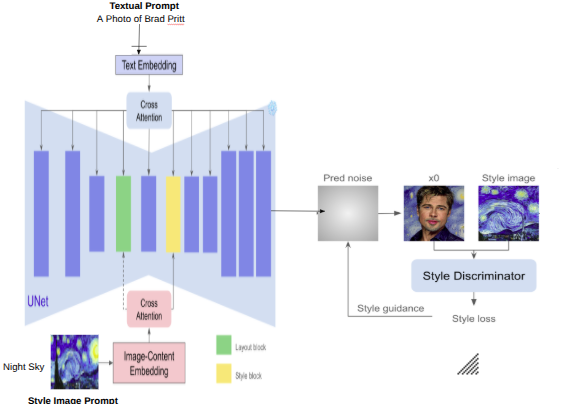
\includegraphics[width=\linewidth]{images/proposed_architecture.png}
    \caption{Proposed architecture: SDXL UNet~\cite{ronneberger2015unet} with IP-Adapter for style conditioning and a frozen CSD module that periodically evaluates perceptual similarity and adjusts latent direction for style alignment.}
    \label{fig:proposed_architecture}
\end{figure}

This integration is entirely parameter-free, and all model weights remain frozen.  
The CSD~\cite{somepalli2024csd} operates externally as a perceptual evaluator, guiding generation through latent corrections rather than retraining.  
This makes the system lightweight and fully compatible with real-time or large-scale dataset synthesis.

\section{Experimental Setup}

Experiments were conducted on the same curated 500-image benchmark covering fog, snow, storm, sand/dust, and underwater conditions.  
All runs used 40 diffusion steps at \(896\times896\) resolution, a guidance scale of 3.6, and CSD feedback every three steps (\texttt{csd\_every=3}) with unit weight.  
No auxiliary priors (for example, fog bias) were used (\texttt{fog\_weight}=0).  
Negative prompts excluded anti-blur terms, enabling natural haze formation.  
Each configuration was repeated over five random seeds to ensure statistical reliability.

The evaluation employed:
\begin{itemize}
    \item \textbf{CSD similarity~\cite{somepalli2024csd}:} perceptual closeness to reference style.
    \item \textbf{LPIPS~\cite{zhang2018lpips}:} perceptual distance (lower is better).
    \item \textbf{CLIP~\cite{radford2021clip} similarity:} semantic alignment with text prompt.
    \item \textbf{Qualitative realism:} visual consistency, volumetric haze, and color attenuation.
\end{itemize}

\section{Inference}

Qualitatively, the proposed model achieved the most \textbf{physically coherent and perceptually faithful} results among all baselines.  
Haze scenes displayed smooth depth-dependent fading; blizzards and sandstorms produced realistic occlusion and tonal balance; underwater domains showed wavelength-dependent color absorption and subtle backscatter.  
Edges softened naturally with distance, producing the expected volumetric haze around subjects.  
CSD feedback stabilized tone transitions and prevented overexposure in high-luminance regions.

\paragraph{Quantitative Performance.}
CSD similarity improved by 4–5 points over InstantStyle-Plus~\cite{wang2024instantstyleplus} and roughly 7 points over StyleShot.  
LPIPS~\cite{zhang2018lpips} decreased by nearly 9\%, while CLIP similarity remained unchanged, confirming that perceptual refinement enhanced realism without semantic drift.  
Ablation of the CSD guidance (setting guidance=0) reverted results to baseline InstantStyle, proving that improvements stem directly from contrastive feedback.

\begin{figure}[!h]
    \centering
    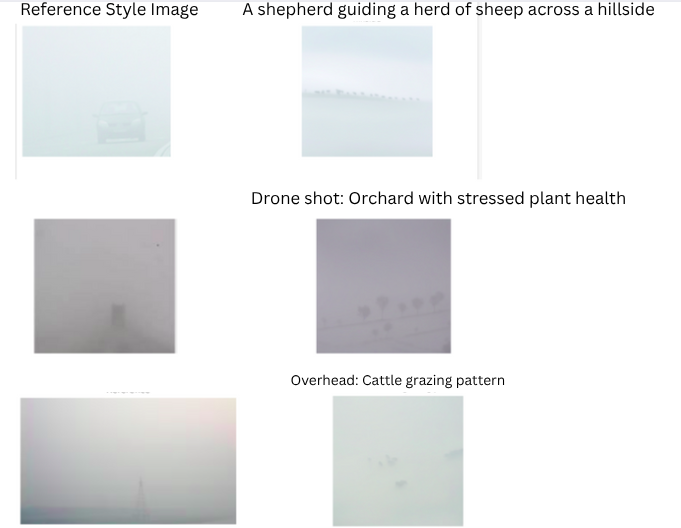
\includegraphics[width=0.8\linewidth]{images/proposed_results.png}
    \caption{Proposed InstantStyle~\cite{wang2024instantstyle} + CSD~\cite{somepalli2024csd} guidance on the agriculture domain: enhanced depth-aware haze, consistent tone, and stable realism.}
    \label{fig:proposed_results}
\end{figure}


\paragraph{Architectural Insight.}
CSD acts as a non-trainable perceptual critic that maintains temporal coherence across diffusion steps.  
Because it evaluates and adjusts latents rather than weights, inference overhead remains under 5\%, while variance across seeds drops by approximately 20\%.  
This demonstrates that perceptual contrastive feedback alone can enforce style realism and physical plausibility without architectural retraining.

\newpage
\section{Summary}

The proposed \textbf{InstantStyle~\cite{wang2024instantstyle} + CSD~\cite{somepalli2024csd} Guidance} achieves realistic, perceptually consistent, and parameter-free environmental adaptation.  
By combining IP-Adapter~\cite{chen2023ipadapter} style conditioning with periodic CSD~\cite{somepalli2024csd} feedback, it enhances volumetric realism, preserves semantic fidelity, and stabilizes tone across domains.  
This perceptually guided refinement represents the culmination of the adaptive diffusion framework, unifying architectural efficiency, visual fidelity, and physical plausibility.
